\documentclass[a4paper,10pt]{article}

\usepackage{datetime}
\usepackage{fullpage}
\usepackage{indentfirst}
\usepackage{amsmath}
\usepackage{amsfonts}
\usepackage{amssymb}
\usepackage{bm}
\usepackage{enumerate}
\usepackage{listings}
\usepackage{graphicx}
\usepackage{float}
\usepackage{multirow}

\linespread{1.5}

\begin{document}
\title{Experiments - Homework 5 \\
  \large Computer Vision (2016 Spring)}
\author{2009-11744 Gyumin Sim}
\maketitle

\section*{Results}

This is the result of the classification with default parameters.
\begin{lstlisting}[language={},frame=single,basicstyle=\small]
     Iteration  Func-count   Grad-count         f(x)         Step-size
         0           1           1             1.38708    
         1           4           2             1.28633               5
         2           7           3             1.08911               1
         3          12           4             1.02919        0.262177
         4          15           5            0.878208               1
         5          18           6            0.833992               1
         6          23           7            0.822577        0.411778
         7          26           8            0.802736               1
         8          29           9            0.791184               1
         9          32          10            0.768214               1
        10          35          11            0.704925               1
       ...         ...         ...                 ...             ...
       140         451         141            0.468264               1
       141         456         142            0.468264        0.391514
       142         459         143            0.468264               1
       143         462         144            0.468264               1
       144         465         145            0.468264               1
    Optimizer Results
        Algorithm Used: limited memory BFGS (L-BFGS)
        Exit message : Change in the objective function value was less than
                       the specified tolerance TolFun.
        iterations : 145
        Function Count : 468
        Minimum found : 0.46826
        Intern Time : 0.9965 seconds
        Total Time : 6.2903 seconds
Accuracy: 80.406%
\end{lstlisting}
It took 2,110 seconds to convolve and pool with the dataset.
$f(x)$ means softmax cost, and the result shows the cost for each iteration.
It ended with 145 iterations because the change in the cost was less than the default tolerance.
The accuracy was $80.406\%$, and the confusion matrix was like Figure \ref{fig:confusion}.
The correspoding labels were airplane, car, cat, and dog in order.
As it can be seen in the confusion matrix, cat and dog are most hard to classify.
\begin{figure}[h]
\caption{Confusion Matrix}
\label{fig:confusion}
\centering
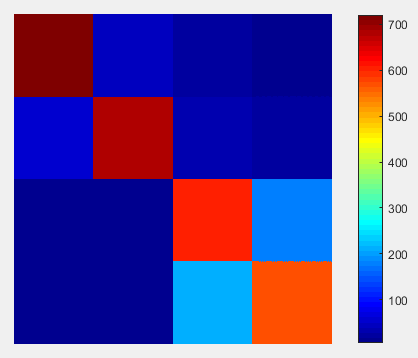
\includegraphics[width=0.5\textwidth]{confusion}
\end{figure}

\section*{Changing Parameters}

Since features are given in \texttt{STL10Features.mat}, there are few chances to change parameters.
I have changed the size of pooling (\texttt{poolDim}), the method of pooling (\texttt{mean} and \texttt{max}), and the weight decay parameter (\texttt{lambda}) for softmax.
The default setting of parameters is that \texttt{poolDim} is $19$, the method of pooling is \texttt{mean}, and \texttt{lambda} is $10^{-4}$.

When it reduced \texttt{poolDim} to $12$, it took more iterations to converge and the converged cost was less (see Figure \ref{fig:cost}), but the accuracy ($79.750\%$) was less than the default setting (see Figure \ref{fig:accuracy}).
When it used \texttt{max} pooling, it took the most iterations to converge, but the accuracy ($78.219\%$) was not good.
For \texttt{lambda}, it converges slowly if \texttt{lambda} is small.
When it reduced \texttt{lambda} to $10^{-5}$, the accuracy ($80.781\%$) was slightly improved.

\begin{figure}[h]
\caption{Cost over iterations}
\label{fig:cost}
\centering
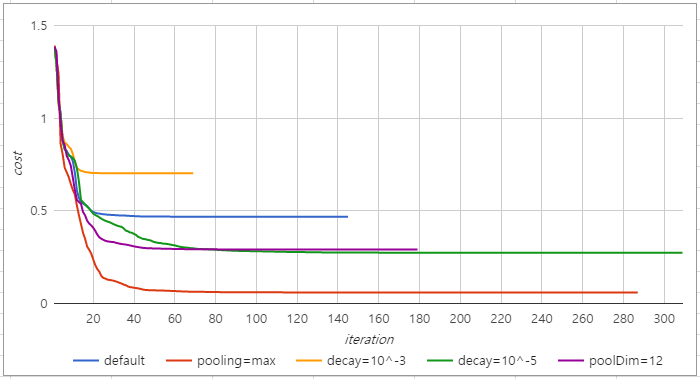
\includegraphics[width=0.9\textwidth]{cost}
\end{figure}

\begin{figure}[h]
\caption{Accuracy with different parameters}
\label{fig:accuracy}
\centering
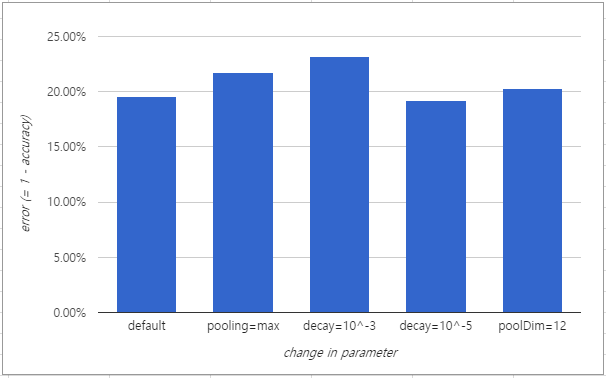
\includegraphics[width=0.8\textwidth]{accuracy}
\end{figure}

\end{document}
